%
% General structure for the revdetua class:
%
\documentclass[shortpaper,english]{revdetua}
%
% Valid options are:
%
%   longpaper --------- \part and \tableofcontents defined
%   shortpaper -------- \part and \tableofcontents not defined (default)
%
%   english ----------- main language is English (default)
%   portugues --------- main language is Portuguese
%
%   draft ------------- draft version
%   final ------------- final version (default)
%
%   times ------------- use times (postscript) fonts for text
%
%   mirror ------------ prints a mirror image of the paper (with dvips)
%
%   visiblelabels ----- \SL, \SN, \SP, \EL, \EN, etc. defined
%   invisiblelabels --- \SL, \SN, \SP, \EL, \EN, etc. not defined (default)
%
% Note: the final version should use the times fonts
% Note: the really final version should also use the mirror option
%

\usepackage{amsmath,hyperref}


\begin{document}

\Header{1}{1}{Novembro}{2022}{1}
% Note: the month must be in Portuguese

\title{Minimum Weight Dominating Set}
\author{Manuel Gomes, 88939} % or \author{... \and ...}
\maketitle

\begin{abstract}% Note: in English
  ...
\end{abstract}

\begin{resumo}% Note: in Portuguese
  ...
\end{resumo}

% \begin{keywords}% Note: in English (optional)
%   ...
% \end{keywords}

% \begin{palavraschave}% Note: in Portuguese (optional)
%   ...
% \end{palavraschave}


\section{Introduction}\label{section:introduction}
Consider a finite, undirected graph $G(V,E)$ , where $V$ is the set of graph vertices and $E$ is the set of graph edges.
Two vertices $u, v$ of $G$ connected by edge $(u,v)$ are called adjacent nodes.
Two edges which share a vertex are also called adjacent.
One edge \emph{dominates} its adjacent.
A set of edges $M$ of $G$ is called an \emph{edge dominating set} if all edges of set $E - M$ are adjacent, and thus dominated, by the edges of $M$ \cite{dominating}.
The weight of an edge dominating set is the sum of its edges' weight. 
A \emph{minimum weight edge dominating set} is an edge dominating set whose total weight is as small as possible.

The objective behind this report is to apply exhaustive search and greedy algorithms to retrieve the minimum weight edge dominating set for a general graph $G$.
The report is divided in five section: the first (\autoref{section:introduction}), where the problem is introduced;
the second (\autoref{section:algorithms-used}), where the algorithms used are described;
the third (\autoref{section:formal-analysis}), where a formal analysis for the algorithms is presented;
the fourth (\autoref{section:results}), where results for experiments conducted with the algorithms are detailed;
and the fifth (\autoref{section:conclusions}), where conclusions are extracted.
\section{Algorithms Used}\label{section:algorithms-used}
To retrieve the minimum weight dominating set of a graph $G$, two different types of algorithm were used.
The first algorithm was an exhaustive search algorithm, while the rest followed a greedy heuristics.

\subsection{Exhaustive Search}\label{section:exhaustive-search}

Exhaustive search is a brute-force approach to combinatorial problems that consists of generating every element of the problem domain, verify if it fulfils a specific condition and then finding a desired element \cite{levitin2012introduction}.

The exhaustive search used for the problem at hand is based on generating every possible combination of edges of the graph.
Then, for every single combination, verify it is a dominating set.
If so, compute the sum of weights of every edge that belongs to the combination.
Then, compare that sum with the current minimum weight.
If the sum is smaller than the minimum, the combination is a better solution than the current minimum set.
Therefore, the combination at hand is the now the current best solution and the sum of the weights is the current minimum weight.
This algorithm is better illustrated in \autoref{alg:exhaustive}.

\begin{algorithm}
\caption{Exhaustive search algorithm}
\label{alg:exhaustive}
\begin{algorithmic}
\Inputs{$G(V,E) \gets$ graph with set of vertices $V$ and set of edges $E$}
\Initialize{$l_c \gets$ list of every combination of edges in $E$

$w_{min} \gets \infty$

$set_{min} \gets [\cdot]$}

\For{$c$ in $l_c$}
    \If{$c$ is dominating set of $G(V,E)$}

        $w_c = \sum$ weight of edges in $c$
        
        \If{$w_c < w_{min}$}

           \State $w_{min} \gets w_c$
           \State $set_{min} \gets c$

        \EndIf        
    \EndIf

\EndFor

\end{algorithmic}
\end{algorithm}

\subsection{Greedy Heuristics}
A greedy approach is a general design technique applicable to optimization problems.
It consists a solution through a set of steps, expanding a partially constructed solution along them.
On each step, a choice need to take place.
That choice needs to be: feasible, so it satisfies the problem's constraints; locally optimal, i.e., it has to be the best possible choice among all feasible choices available; and irreversible, i.e., the choice, once made, cannot be changed \cite{levitin2012introduction}.

For the current problem, three different greedy heuristics were developed: minimum weight, maximum connection and one based on the work of Chaurasia and Singh\cite{chaurasia}.

In the first one, edges of the graph are sorted in ascending order by weight. 
Then, the edge with the least weight is added to the solution set.
The solution set is checked to verify if it is a dominating set.
If so, the solution is found and the algorithm stops.
If not, add the next edge to the solution edge.
The algorithm is described in \autoref{alg:min-weight}. 

\begin{algorithm}
\caption{Minimum weight greedy heuristics}
\label{alg:min-weight}
\begin{algorithmic}
\Inputs{$G(V,E) \gets$ graph with set of vertices $V$ and set of edges $E$}
\Initialize{$l_{E,W} \gets$ list of $E$ with corresponding set of weights $W$

$w_{min} \gets 0$

$set_{min} \gets [\cdot]$}


\State $l_{E,W-sorted} = l_{E,W}$ sorted in ascending order by weight
\For{$edge,\ weight$ in $l_{E,W-sorted}$}

    \State $set_{min} \gets$ add $edge$
    \State $w_{min} += weight$
    \If{$set_{min}$ is dominating set of $G(V,E)$}

        \State \textbf{break}
    \EndIf
\EndFor
\end{algorithmic}
\end{algorithm}

The second one is similar to the first, with the difference lying in the sorting step.
Instead of sorting in ascending order by weight, this heuristics sorts the edges in descending order by number of adjacent edges, as seen in \autoref{alg:max-connection}.

\begin{algorithm}
\caption{Maximum connection greedy heuristics}
\label{alg:max-connection}
\begin{algorithmic}
\Inputs{$G(V,E) \gets$ graph with set of vertices $V$ and set of edges $E$}
\Initialize{$l_{E,W,NA} \gets$ list of $E$ with corresponding sets of weights $W$ and of the number of adjacent edges $NA$

$w_{min} \gets 0$

$set_{min} \gets [\cdot]$}


\State $l_{E,W,NA-sorted} = l_{E,W,NA}$ sorted in descending order by number of adjacent edges
\For{$edge,\ weight,\ n_{adjacent}$ in $l_{E,W,NA-sorted}$}

    \State $set_{min} \gets$ add $edge$
    \State $w_{min} += weight$
    \If{$set_{min}$ is dominating set of $G(V,E)$}

        \State \textbf{break}
    \EndIf
\EndFor
\end{algorithmic}
\end{algorithm}

% \newpage
The third greedy algorithm is based on the work by Chaurasia-Singh\cite{chaurasia}.
In this algorithm, a weight ratio for a certain edge is calculated by dividing the sum of the weights of its adjacent edges with its weight.
The edges are then sorted in descending order by their weight ratio.
The algorithm is exemplified in \autoref{alg:chaurasia}.

\newpage

\begin{algorithm}
\caption{Chaurasia-Singh greedy heuristics}
\label{alg:chaurasia}
\begin{algorithmic}
\Inputs{$G(V,E) \gets$ graph with set of vertices $V$ and set of edges $E$}
\Initialize{$l_{E,W,A,W_{A}} \gets$ list of $E$ with corresponding sets of weights $W$, of adjacent edges $A$ and of weight of adjacent edges $W_A$}

$w_{min} \gets 0$

$set_{min} \gets [\cdot]$

$l_{W_{r} \gets [\cdot]}$

\For{$edge,\ weight,\ edges_{adjacents}, weight_{adjacents}$ in $l_{E,W,A,W_{A}}$}
    
    $W_{ratio} = weight_{adjacents} / weight$
    \State $l_{W_{r}} \gets$ add $W_{ratio}$

\EndFor

\State $l_{E,W,A,W_{A},W_{r}} \gets [l_{E,W,A,W_{A}},\ l_{W_{r}}]$

\State $l_{E,W,A,W_{A},W_{r}-sorted} = l_{E,W,A, W_{A}, W_{r}}$ sorted in descending order by weight ratio $w_r$
\For{$edge,\ weight,\ edges_{adjacent},\ weight_{adjacent}, weight_{ratio}$ in $l_{E-W-Asorted}$}

    \State $set_{min} \gets$ add $edge$
    \State $w_{min} += weight$
    \If{$set_{min}$ is dominating set of $G(V,E)$}

        \State \textbf{break}
    \EndIf
\EndFor
\end{algorithmic}
\end{algorithm}
\section{Formal Analysis}\label{section:formal-analysis}
This section will be focused on performing a formal analysis for the algorithm described in \autoref{section:algorithms-used}.
This formal analysis will consist of presenting their basic operations, defining a closed formula for the number of basic operations, their order of growth, and the worst and best cases.

For the exhaustive search algorithm, the basic operation defined is verifying if a set is a dominating set, due to their repetitiveness.
This operation takes place for every combination of edges in a graph.
For a generic graph $G(V,E)$ with $m$ vertices and $n$ edges, the combination of edges can be given by a set of binary number with $n$ elements.
Every binary number corresponds to a certain edge. 
When it is zero, the edge is not present in the combination.
When it is one, the edge is present in the combination.
This concept is better illustrated by \autoref{eq:edges} and \autoref{eq:combination}.

\begin{equation}
    edges = [e_1,\ e_2,\ ...,\ e_(n-1),\ e_n]
    \label{eq:edges}
\end{equation}

\begin{equation}
    combination = [0,\ 1,\ ...,\ 1,\ 0],\ \text{with length }n
    \label{eq:combination}
\end{equation}

So, if every combination can be defined by a set of binary numbers with length $n$, it can be concluded that the closed formula for the number of basic operations is given by \autoref{eq:ex-closed-formula}.

\begin{equation}
    T(n) = 2^n
    \label{eq:ex-closed-formula}
\end{equation}

Therefore, we conclude the order of magnitude of the algorithm is exponential, as seen in \autoref{eq:ex-big-o}.

\begin{equation}
    O(n) = 2^n
    \label{eq:ex-big-o}
\end{equation}

As the algorithm always needs to verify every single combination, the best and worst case scenario are given by \autoref{eq:ex-worst} and \autoref{eq:ex-best}.

\begin{equation}
    W(n) = 2^n
    \label{eq:ex-worst}
\end{equation}
\begin{equation}
    B(n) = 2^n
    \label{eq:ex-best}
\end{equation}

For the greedy heuristics, the basic operation defined is the sorting of the lists of edges, due to behind the most time consuming operation.
The sorting algorithm used was the \verb|sort()| function in Python 3, which according to documentation \cite{sortpython}, has a order of magnitude given by \autoref{eq:greedy-big-o}.

\begin{equation}
    O(n) = nlog_2(n)
    \label{eq:greedy-big-o}
\end{equation}

Regarding the best and worst case scenario, the algorithm can found an adequate solution after one iteration or after iterating for every edge.
Therefore, the best and worst cases can be defined by \autoref{eq:greedy-worst} and \autoref{eq:greedy-best}.

\begin{equation}
    W(n) = n
    \label{eq:greedy-worst}
\end{equation}
\begin{equation}
    B(n) = 1
    \label{eq:greedy-best}
\end{equation}
\section{Results}\label{section:results}
After implementing the algorithms described in \autoref{section:algorithms-used}, experimental results were retrieved.
These results range from number of operation, elapsed time and relative error.
The results were taken in a machine with the AMD Ryzen 5 5600X processor.

For the exhaustive search algorithm, the results obtained are presented in \autoref{tab:ex-table}, \autoref{fig:ex-op}, and \autoref{fig:ex-time}.
In \autoref{tab:ex-table}, $V$ and $E$ are the number of vertices and edges of the graph; $p$ is the fraction between $E$ and the maximum number of edges; execution time is the time elapsed during the computation of the algorithm;
number of basic operations is how many basic operations (defined in \autoref{section:formal-analysis}) took place; number of dominating sets is the number of sets generated that were dominating sets; and the time per operation is the estimated elapsed time for a basic operation.
From this data we can verify that the number of basic operations presents an exponential order of growth, following the behavior expected by \autoref{eq:ex-closed-formula} and \autoref{eq:ex-big-o}.
The execution time also presents an exponential growth with the number of edges.
The time per basic operation in seconds is $3,71e\scalebox{0.5}[1.0]{\( - \)}5 \pm 8,36e{\scalebox{0.5}[1.0]{\( - \)}6}$.
From these experiences, the largest graph able to be computed was one with 9 vertices and 23 edges (\autoref{fig:9-05-ex}).
\autoref{eq:ex-time-calc} is used to calculate how long a computation takes using the same hardware.


\begin{table}[ht!]
\caption{Results from exhaustive search algorithm}
\label{tab:ex-table}
\resizebox{0.5\textwidth}{!}{%
\begin{tabular}{ccccccc}
\multirow{3}{*}{V} & \multirow{3}{*}{p} & \multirow{3}{*}{E} & \multirow{3}{*}{\begin{tabular}{c} Execution \\ Time (s) \end{tabular}} & \multirow{3}{*}{\begin{tabular}{c} \# of \\ Basic \\Operations\end{tabular}} & \multirow{3}{*}{\begin{tabular}{c} \# of \\ Dominating \\Sets\end{tabular}} & \multirow{3}{*}{\begin{tabular}{c}Time per \\ Operation (s)\end{tabular}} \\ 
& & & & & & \\
& & & & & & \\
\hline
4 & 0,125 & 4 & 7,89E-04 & 16 & 13 & 5,26E-05 \\
4 & 0,25 & 6 & 2,68E-03 & 64 & 57 & 4,26E-05 \\
4 & 0,5 & 6 & 2,57E-03 & 64 & 57 & 4,07E-05 \\
4 & 0,75 & 6 & 2,76E-03 & 64 & 57 & 4,38E-05 \\
5 & 0,125 & 4 & 6,00E-04 & 16 & 11 & 4,00E-05 \\
5 & 0,25 & 6 & 3,22E-03 & 64 & 49 & 5,11E-05 \\
5 & 0,5 & 7 & 5,12E-03 & 128 & 107 & 4,03E-05 \\
5 & 0,75 & 8 & 1,06E-02 & 256 & 227 & 4,15E-05 \\
6 & 0,125 & 5 & 1,22E-03 & 32 & 21 & 3,93E-05 \\
6 & 0,25 & 8 & 6,64E-03 & 256 & 203 & 2,61E-05 \\
6 & 0,5 & 12 & 1,74E-01 & 4096 & 3835 & 4,24E-05 \\
6 & 0,75 & 13 & 2,33E-01 & 8192 & 7823 & 2,85E-05 \\
7 & 0,125 & 6 & 1,59E-03 & 64 & 33 & 2,53E-05 \\
7 & 0,25 & 10 & 2,76E-02 & 1024 & 871 & 2,70E-05 \\
7 & 0,5 & 15 & 1,21E+00 & 32768 & 31017 & 3,71E-05 \\
7 & 0,75 & 18 & 1,14E+01 & 262144 & 256281 & 4,34E-05 \\
8 & 0,125 & 8 & 6,32E-03 & 256 & 159 & 2,48E-05 \\
8 & 0,25 & 12 & 1,15E-01 & 4096 & 3407 & 2,80E-05 \\
8 & 0,5 & 18 & 9,86E+00 & 262144 & 247957 & 3,76E-05 \\
8 & 0,75 & 23 & 3,51E+02 & 8388608 & 8274471 & 4,19E-05 \\
9 & 0,125 & 10 & 2,63E-02 & 1024 & 731 & 2,57E-05 \\
9 & 0,25 & 17 & 4,03E+00 & 131072 & 118053 & 3,07E-05 \\
9 & 0,5 & 23 & 3,61E+02 & 8388608 & 8064383 & 4,30E-05
\end{tabular}%
}
\end{table}

\newpage

\begin{figure}[!ht]
    \centering
    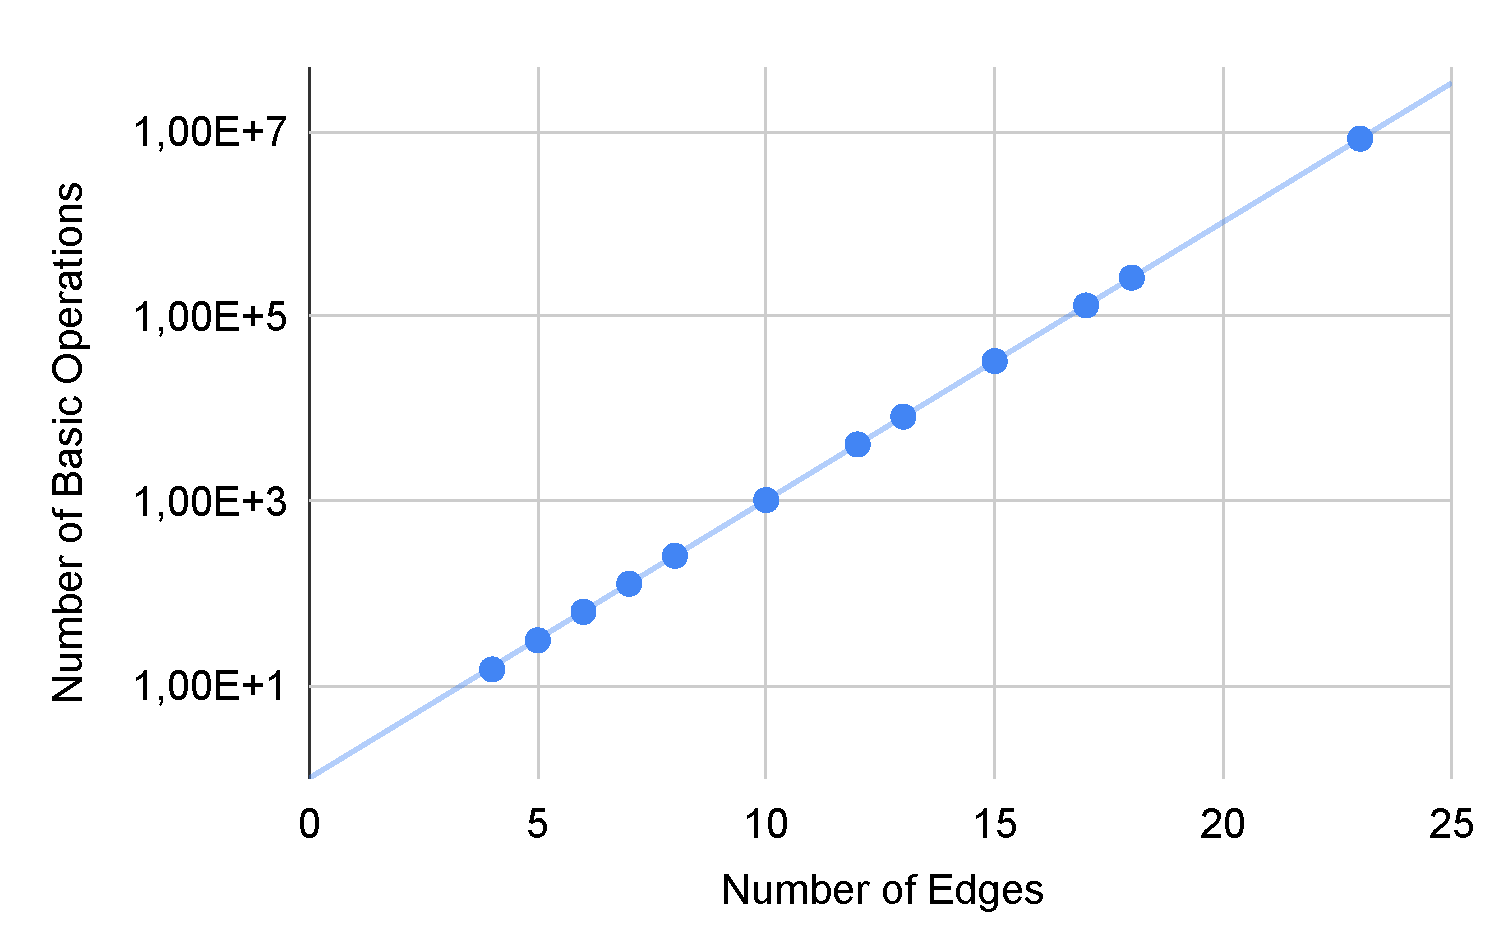
\includegraphics[width=0.9\linewidth]{figs/ex-basic-operations.pdf}
    \caption{Correlation between number of edges and number of basic operation for exhaustive search. Logarithmic scale.}
    \label{fig:ex-op}
\end{figure}

\begin{figure}[!ht]
    \centering
    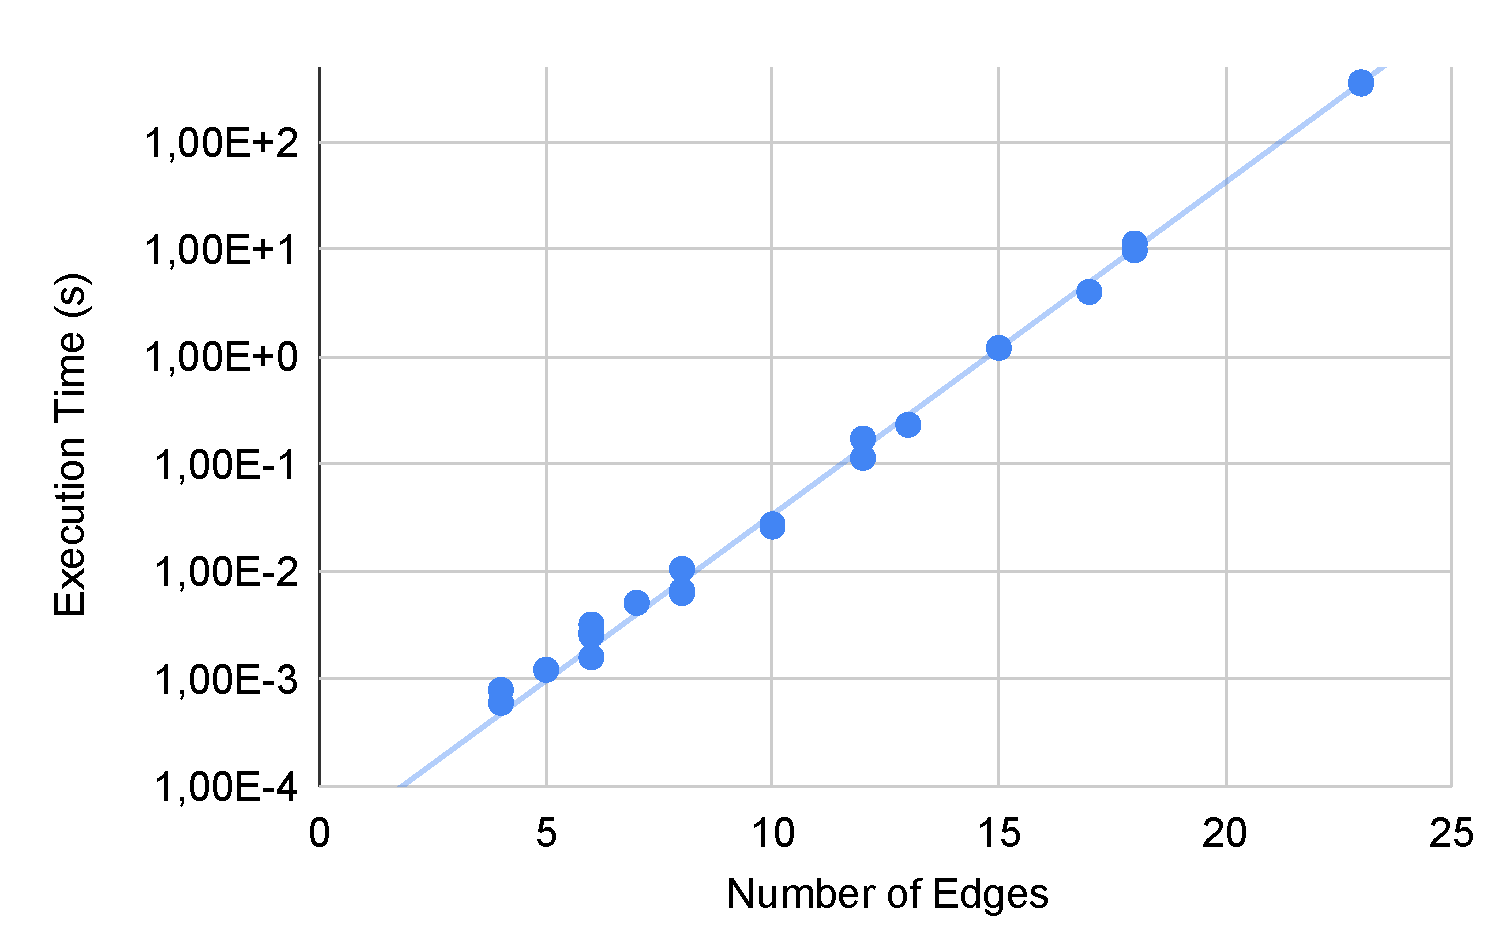
\includegraphics[width=0.9\linewidth]{figs/ex-time.pdf}
    \caption{Correlation between number of edges and elapsed time for exhaustive search. Logarithmic scale.}
    \label{fig:ex-time}
\end{figure}

\begin{figure}[!ht]
    \centering
    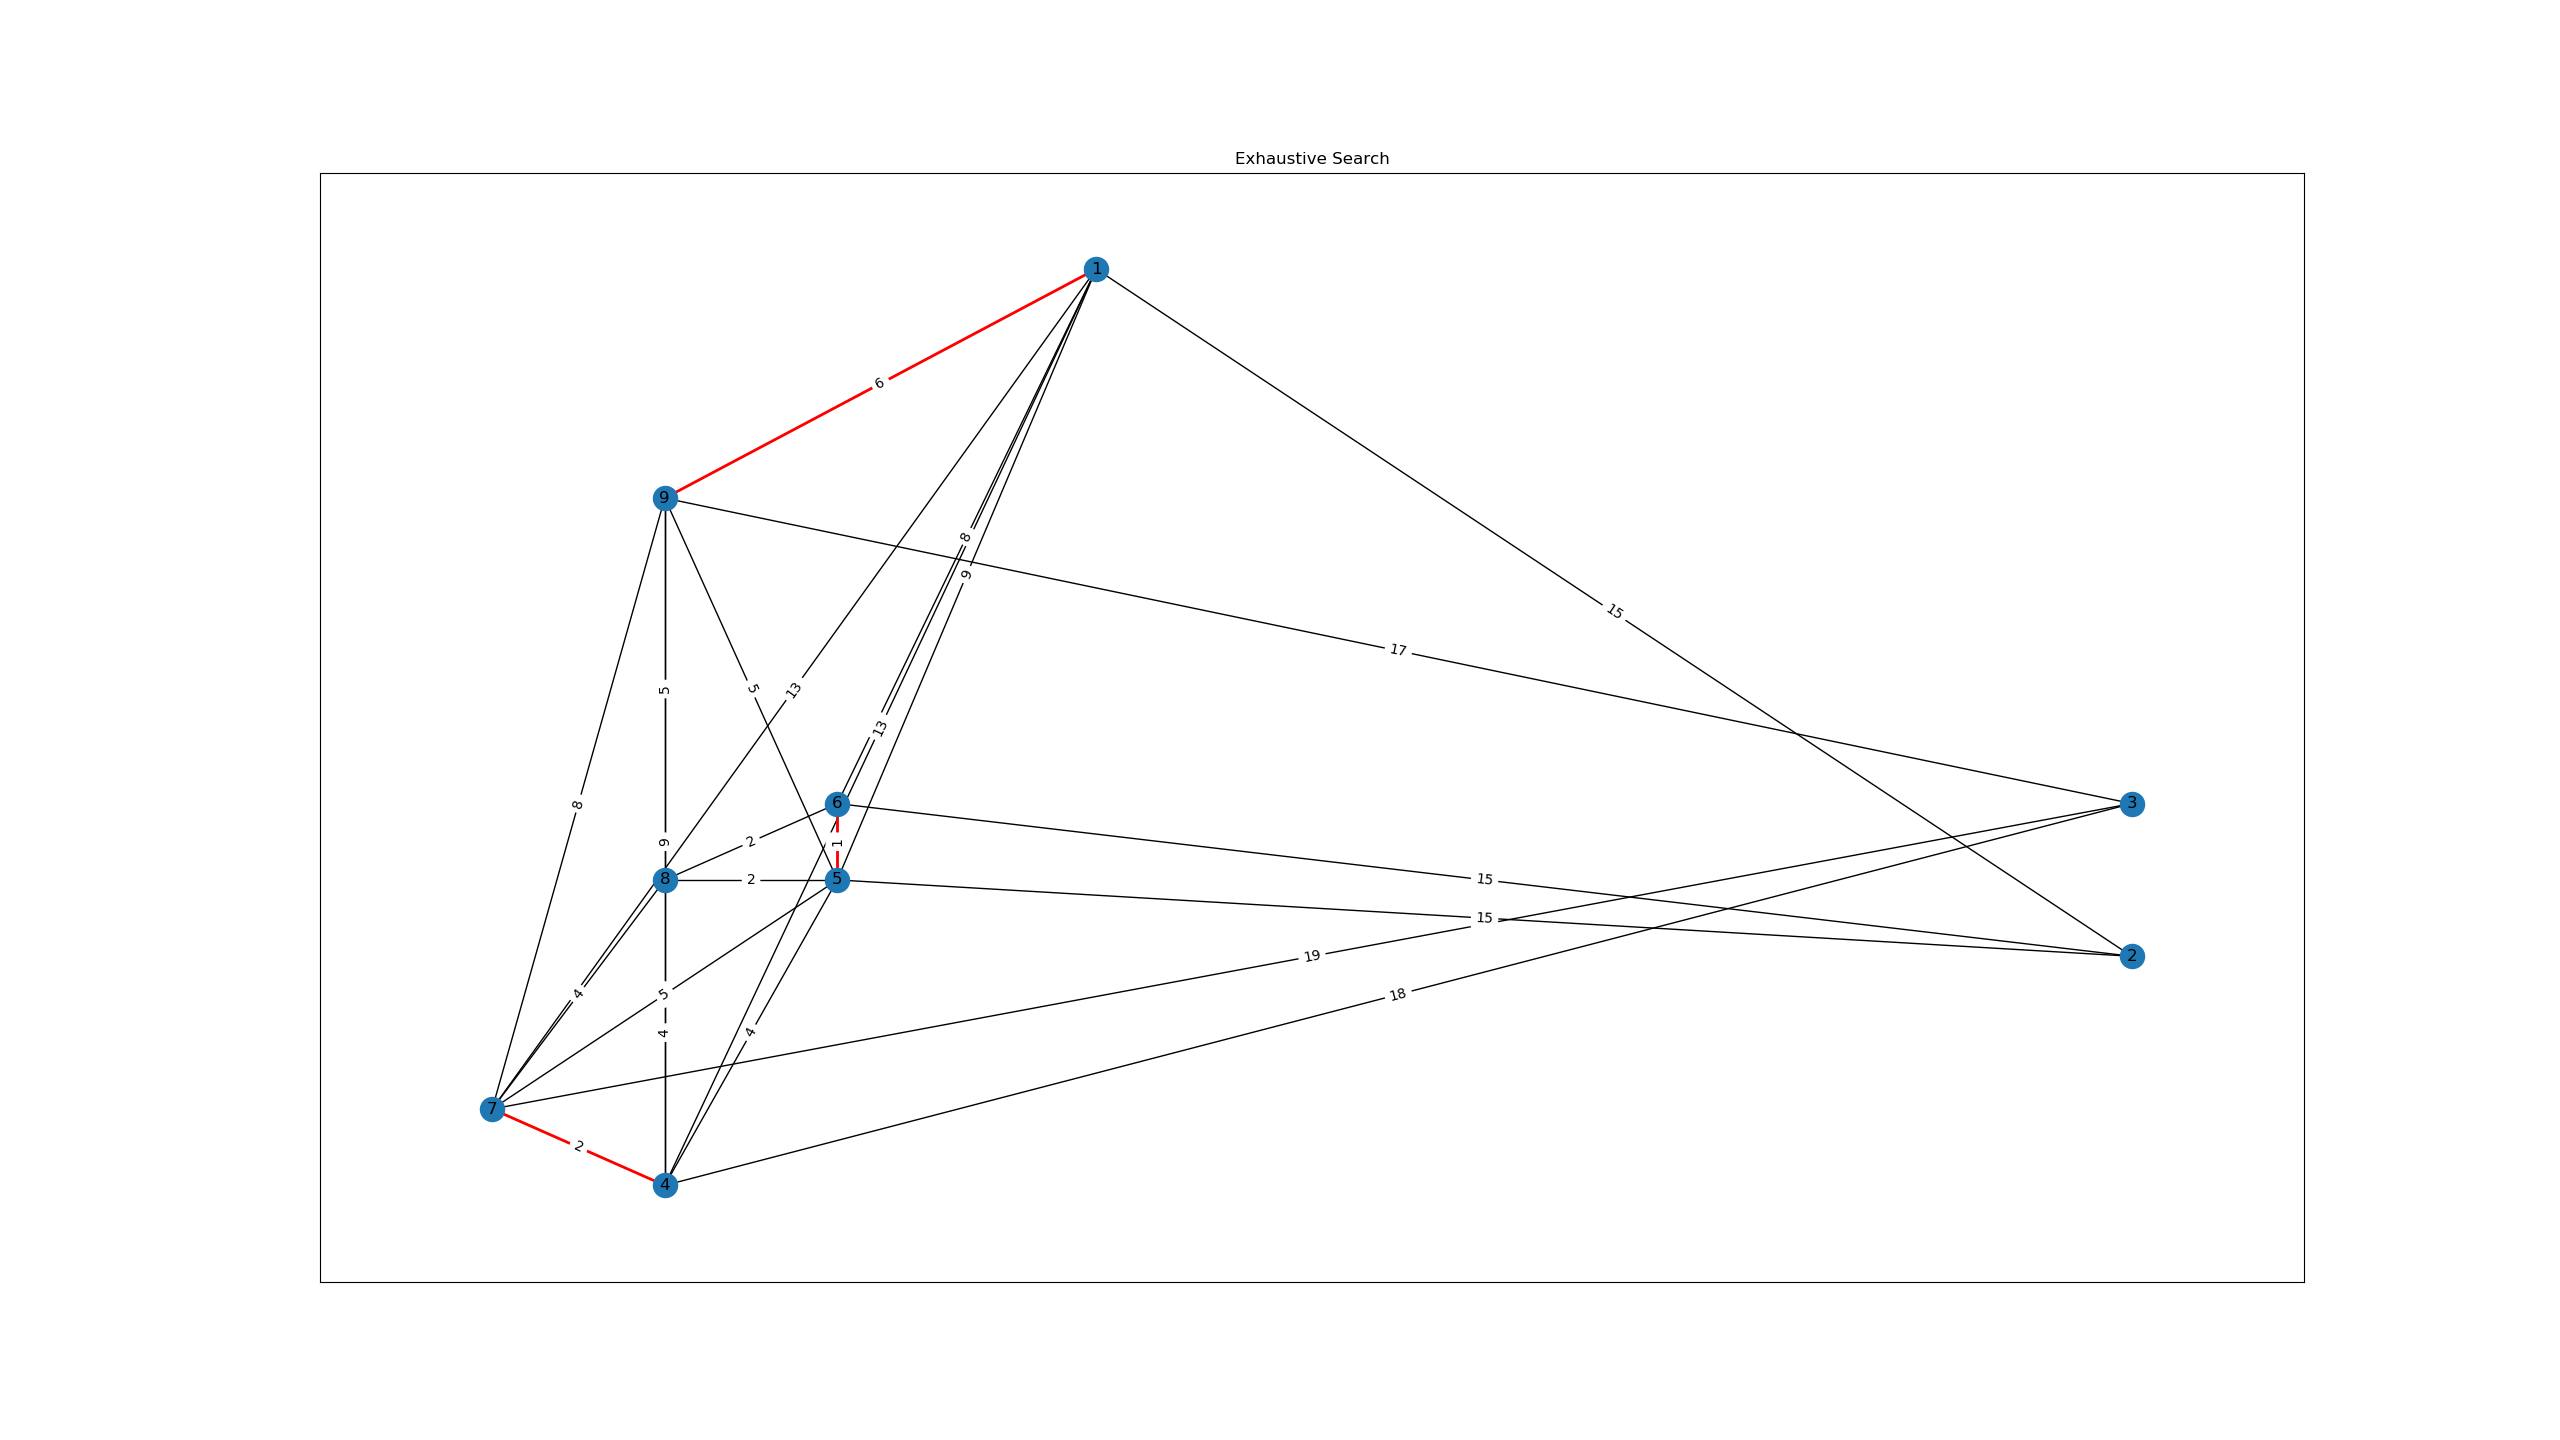
\includegraphics[width=1\linewidth]{figs/fig-9-0.5-exhaustive}
    \caption{Largest graph able to be processed. 9 nodes and 23 edges.}
    \label{fig:9-05-ex}
\end{figure}

\begin{equation}
    time = T(n) * 3,71e\scalebox{0.5}[1.0]{\( - \)}5 = 2^n * 3,71e\scalebox{0.5}[1.0]{\( - \)}5
    \label{eq:ex-time-calc}
\end{equation}

\newpage

For the minimum weight greedy heuristics, the results obtained are presented in \autoref{tab:minw-table}, \autoref{fig:minw-sol}, \autoref{fig:minw-time}, and \autoref{fig:minw-ratio}. 
The columns for \autoref{tab:minw-table} are equal to the ones in \autoref{tab:ex-table}, with the exception of: number of solutions tested, which is the number of sets tested before a dominating one was formed; and accuracy ratio, which is a measure used to compare the weight of the solution obtained with the weight of the optimal solution. 
This data verifies that the number of solutions tested grows with the number of edges.
The correlation between the elapsed time and the number of edges presents a form of a $nlog_2(n)$ function, verifying the hypothesis formed in \autoref{eq:greedy-big-o}.
From the accuracy ratio, it can be inferred that the algorithm is relatively accurate in smaller graph, becoming less accurate in larger graphs.


\begin{table}[ht!]
\caption{Results from minimum weight greedy algorithm}
\label{tab:minw-table}
\resizebox{0.5\textwidth}{!}{%
\begin{tabular}{ccccccc}
\multirow{3}{*}{V} & \multirow{3}{*}{p} & \multirow{3}{*}{E} & \multirow{3}{*}{\begin{tabular}{c} Execution \\ Time (s) \end{tabular}} & \multirow{3}{*}{\begin{tabular}{c}\# of\\ Solutions\\Tested\end{tabular}} & \multirow{3}{*}{\begin{tabular}{c} Accuracy \\ Ratio \end{tabular}}\\ 
& & & & & & \\
& & & & & & \\
\hline
4 & 0.125 & 4 & 1,05E-04 & 2 & 1,80 \\
4 & 0.25 & 6 & 1,03E-04 & 2 & 1,00 \\
4 & 0.5 & 6 & 9,78E-05 & 2 & 1,00 \\
4 & 0.75 & 6 & 1,15E-04 & 2 & 1,00 \\
5 & 0.125 & 4 & 7,20E-05 & 1 & 1,00 \\
5 & 0.25 & 6 & 1,05E-04 & 2 & 1,00 \\
5 & 0.5 & 7 & 9,78E-05 & 2 & 1,00 \\
5 & 0.75 & 8 & 1,08E-04 & 2 & 1,00 \\
6 & 0.125 & 5 & 9,58E-05 & 3 & 1,50 \\
6 & 0.25 & 8 & 1,03E-04 & 4 & 1,61 \\
6 & 0.5 & 12 & 1,05E-04 & 3 & 1,00 \\
6 & 0.75 & 13 & 9,87E-05 & 3 & 1,00 \\
7 & 0.125 & 6 & 8,51E-05 & 3 & 1,00 \\
7 & 0.25 & 10 & 1,11E-04 & 4 & 1,60 \\
7 & 0.5 & 15 & 1,78E-04 & 4 & 1,56 \\
7 & 0.75 & 18 & 2,03E-04 & 4 & 1,27 \\
8 & 0.125 & 8 & 8,85E-05 & 3 & 1,00 \\
8 & 0.25 & 12 & 8,03E-05 & 2 & 1,00 \\
8 & 0.5 & 18 & 1,34E-04 & 4 & 1,31 \\
8 & 0.75 & 23 & 3,10E-04 & 6 & 1,75 \\
9 & 0.125 & 10 & 1,48E-04 & 6 & 2,13 \\
9 & 0.25 & 17 & 1,96E-04 & 7 & 2,56 \\
9 & 0.5 & 23 & 5,75E-04 & 11 & 4,44
\end{tabular}%
}
\end{table}

\begin{figure}[!ht]
    \centering
    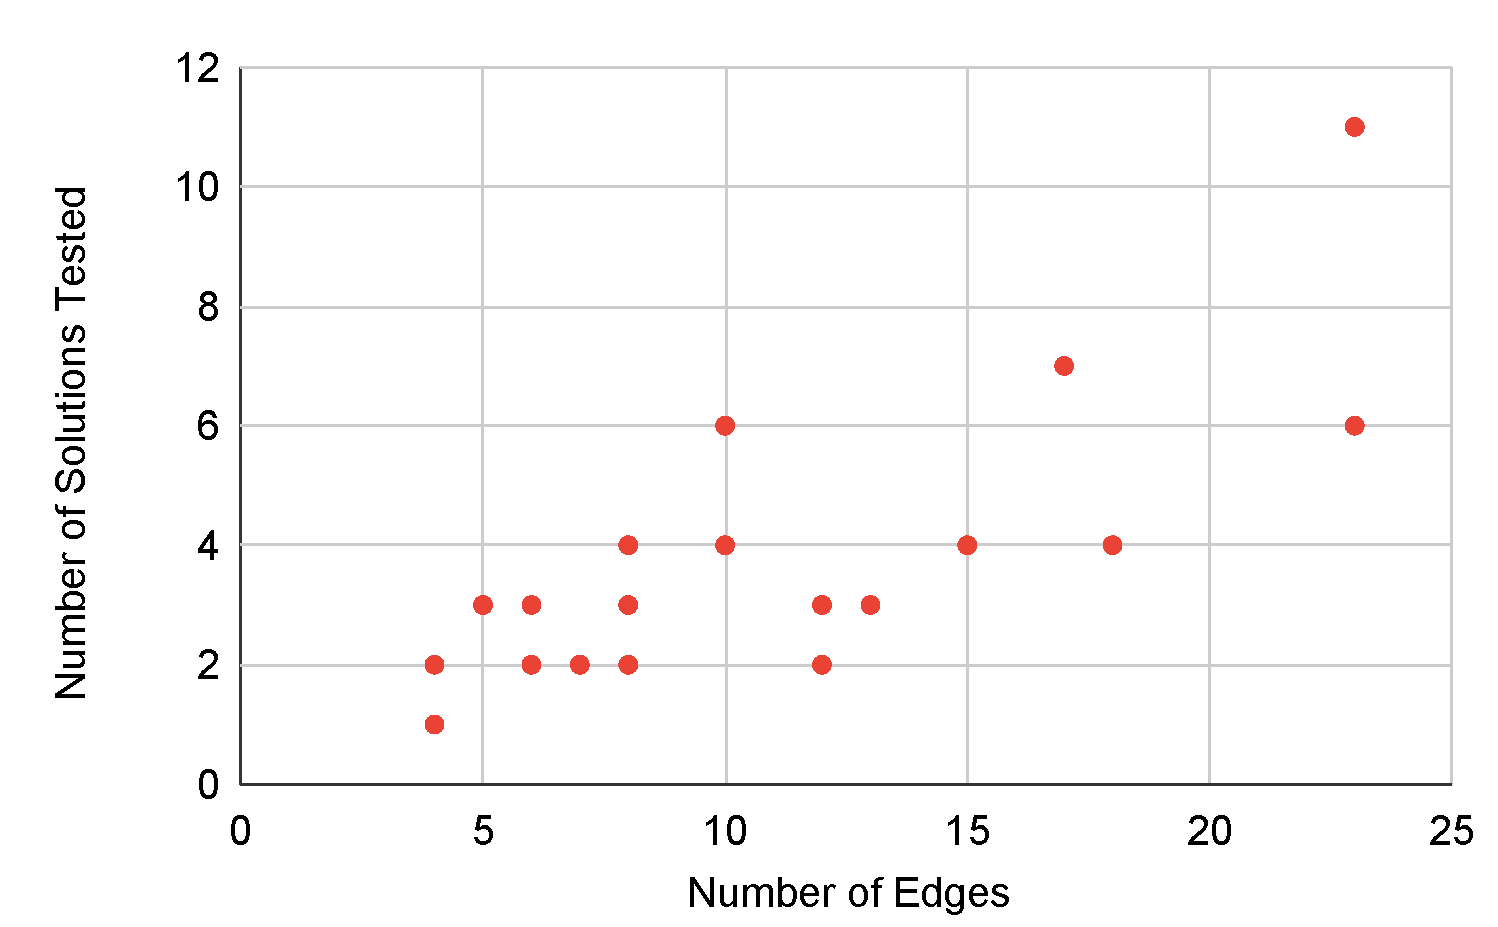
\includegraphics[width=0.9\linewidth]{figs/minw-solutions.pdf}
    \caption{Correlation between number of edges and number of solutions tested for minimum weight greedy algorithm.}
    \label{fig:minw-sol}
\end{figure}


\begin{figure}[!ht]
    \centering
    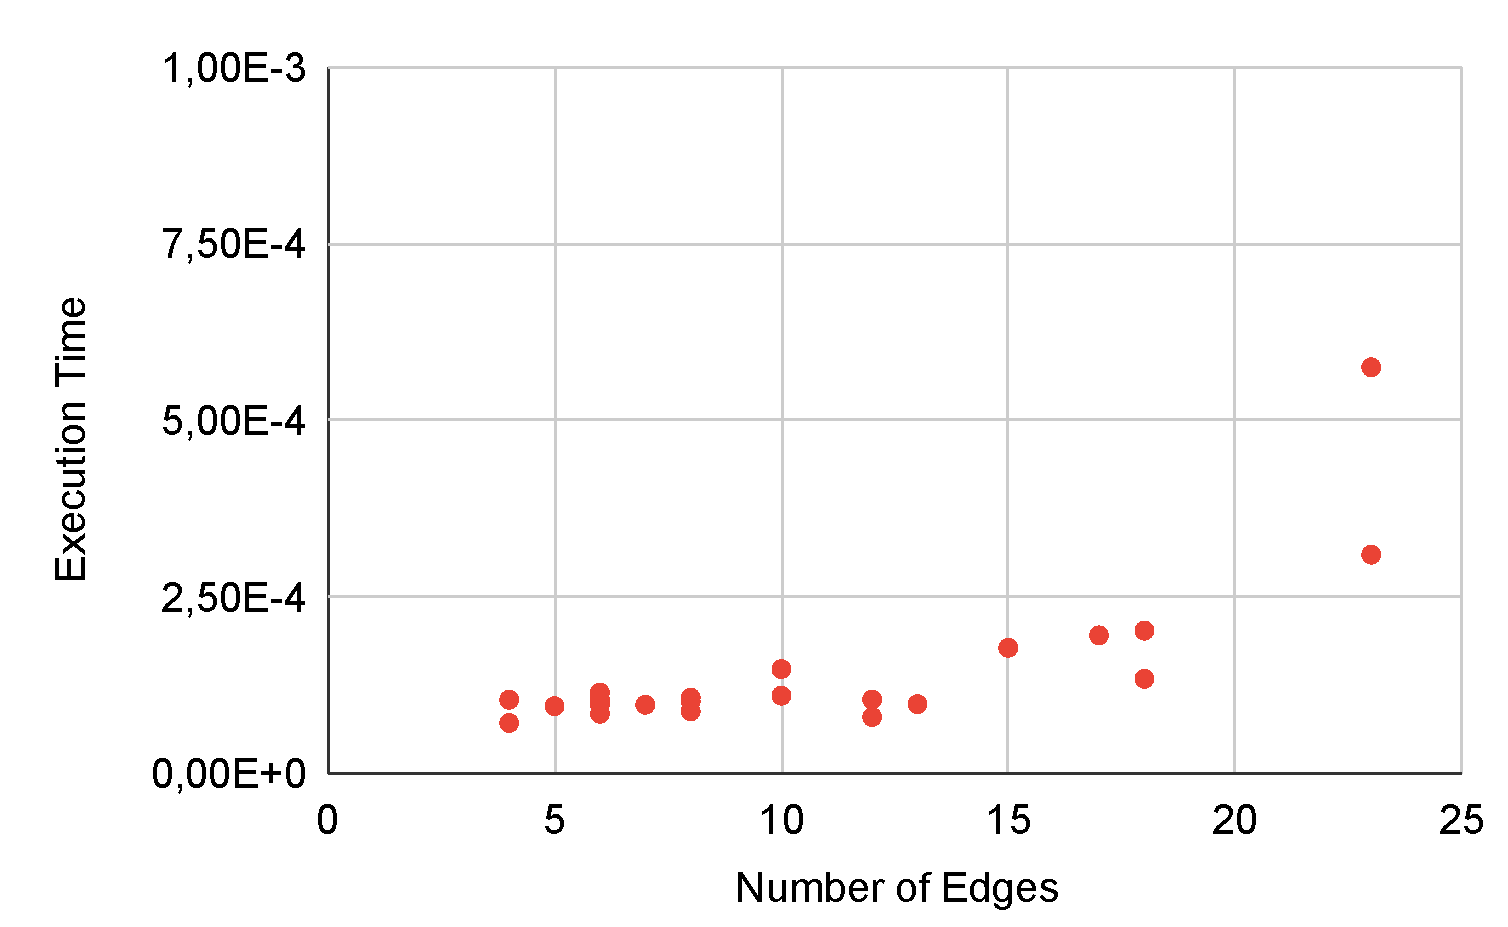
\includegraphics[width=0.9\linewidth]{figs/minw-time.pdf}
    \caption{Correlation between number of edges and elapsed time for minimum weight greedy algorithm.}
    \label{fig:minw-time}
\end{figure}

\newpage

\begin{figure}[!ht]
    \centering
    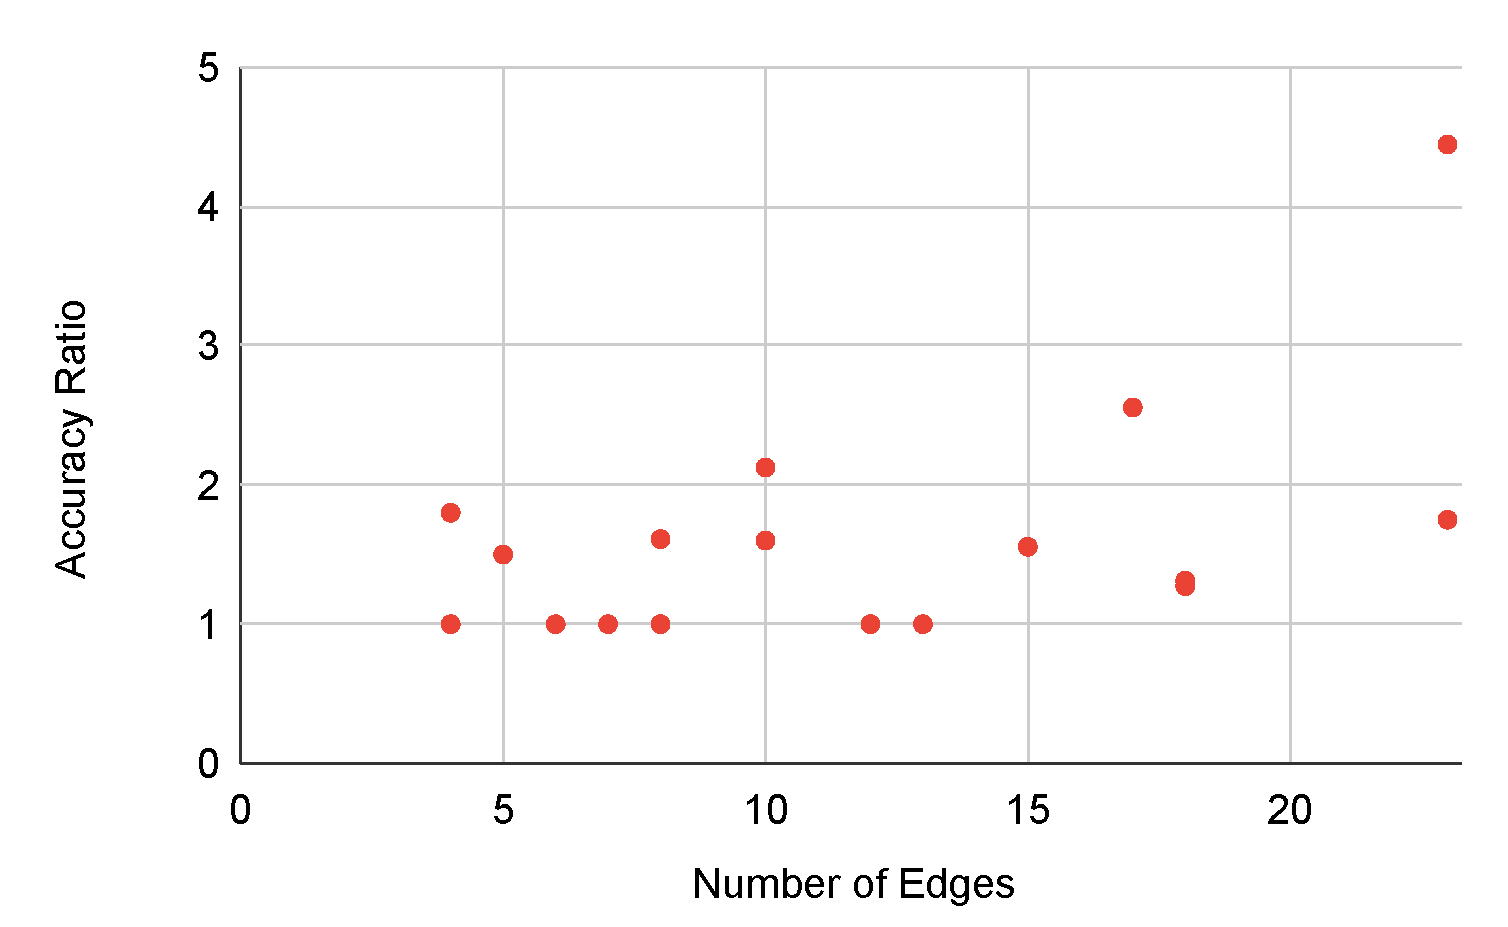
\includegraphics[width=0.9\linewidth]{figs/minw-ratio.pdf}
    \caption{Correlation between number of edges and accuracy ratio for minimum weight greedy algorithm.}
    \label{fig:minw-ratio}
\end{figure}


For the maximum connection greedy heuristics, the results obtained are presented in \autoref{tab:maxc-table}, \autoref{fig:maxc-sol}, \autoref{fig:maxc-time}, and \autoref{fig:maxc-ratio}. 
The columns for \autoref{tab:maxc-table} are equal to the ones in \autoref{tab:minw-table}.
The data shows that the number of solutions tested grows with the number of edges, however, is smaller than the previous heuristics.
As with the previous algorithm, the correlation between the elapsed time and the number of edges presents a form of a $nlog_2(n)$ function, further verifying the hypothesis formed in \autoref{eq:greedy-big-o}.
With the accuracy ratio, it can be stated that the algorithm, although not completely inaccurate, is not particularly accurate in smaller graphs.
However, the inaccuracy does not seem to grow, at least not in a noticeable rate, for larger graphs.

\newpage

\begin{table}[ht!]
\caption{Results from maximum connection greedy algorithm}
\label{tab:maxc-table}
\resizebox{0.5\textwidth}{!}{%
\begin{tabular}{ccccccc}
\multirow{3}{*}{V} & \multirow{3}{*}{p} & \multirow{3}{*}{E} & \multirow{3}{*}{\begin{tabular}{c} Execution \\ Time (s) \end{tabular}} & \multirow{3}{*}{\begin{tabular}{c}\# of\\ Solutions\\Tested\end{tabular}} & \multirow{3}{*}{\begin{tabular}{c} Accuracy \\ Ratio \end{tabular}}\\ 
& & & & & & \\
& & & & & & \\
\hline
4 & 0.125 & 4 & 1,54E-04 & 1 & 1,00 \\
4 & 0.25 & 6 & 2,10E-04 & 2 & 1,13 \\
4 & 0.5 & 6 & 2,15E-04 & 2 & 1,13 \\
4 & 0.75 & 6 & 2,14E-04 & 2 & 1,13 \\
5 & 0.125 & 4 & 1,48E-04 & 1 & 1,00 \\
5 & 0.25 & 6 & 2,12E-04 & 2 & 2,00 \\
5 & 0.5 & 7 & 2,13E-04 & 2 & 1,00 \\
5 & 0.75 & 8 & 2,28E-04 & 2 & 1,08 \\
6 & 0.125 & 5 & 1,73E-04 & 2 & 1,69 \\
6 & 0.25 & 8 & 1,80E-04 & 3 & 1,89 \\
6 & 0.5 & 12 & 2,17E-04 & 3 & 1,36 \\
6 & 0.75 & 13 & 2,31E-04 & 3 & 2,14 \\
7 & 0.125 & 6 & 1,69E-04 & 3 & 1,58 \\
7 & 0.25 & 10 & 2,03E-04 & 2 & 1,80 \\
7 & 0.5 & 15 & 3,58E-04 & 3 & 2,11 \\
7 & 0.75 & 18 & 2,93E-04 & 3 & 1,27 \\
8 & 0.125 & 8 & 1,61E-04 & 2 & 1,35 \\
8 & 0.25 & 12 & 2,19E-04 & 3 & 3,27 \\
8 & 0.5 & 18 & 2,86E-04 & 4 & 2,06 \\
8 & 0.75 & 23 & 4,77E-04 & 3 & 1,19 \\
9 & 0.125 & 10 & 2,01E-04 & 3 & 1,63 \\
9 & 0.25 & 17 & 2,55E-04 & 3 & 1,44 \\
9 & 0.5 & 23 & 6,18E-04 & 4 & 3,22
\end{tabular}%
}
\end{table}

\begin{figure}[!ht]
    \centering
    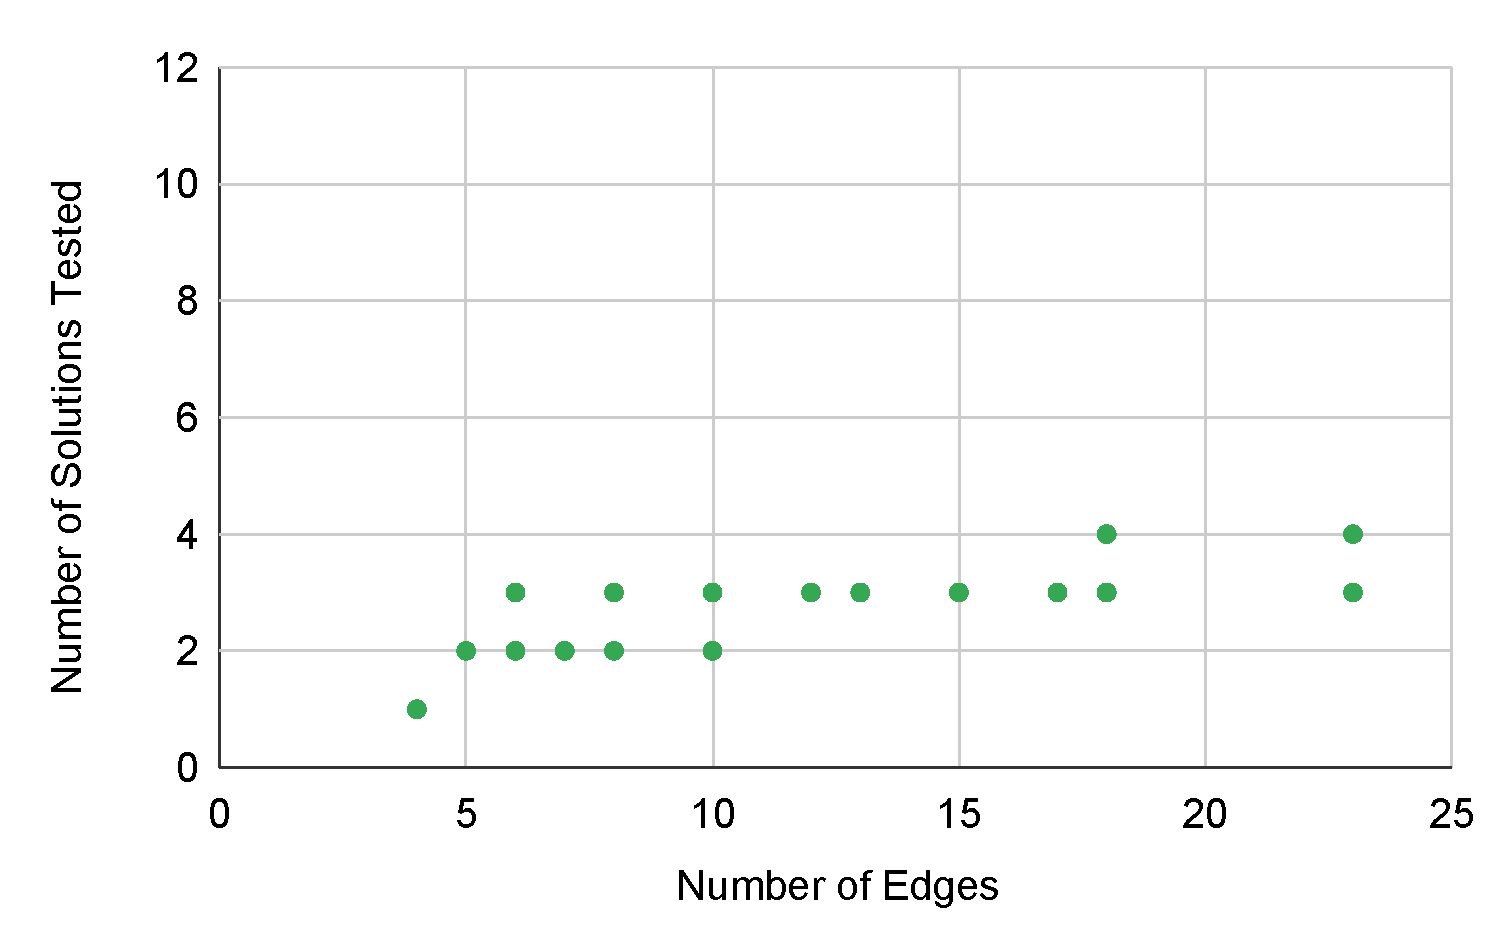
\includegraphics[width=0.9\linewidth]{figs/maxc-solutions.pdf}
    \caption{Correlation between number of edges and number of solutions tested for maximum connection greedy algorithm.}
    \label{fig:maxc-sol}
\end{figure}


\begin{figure}[!ht]
    \centering
    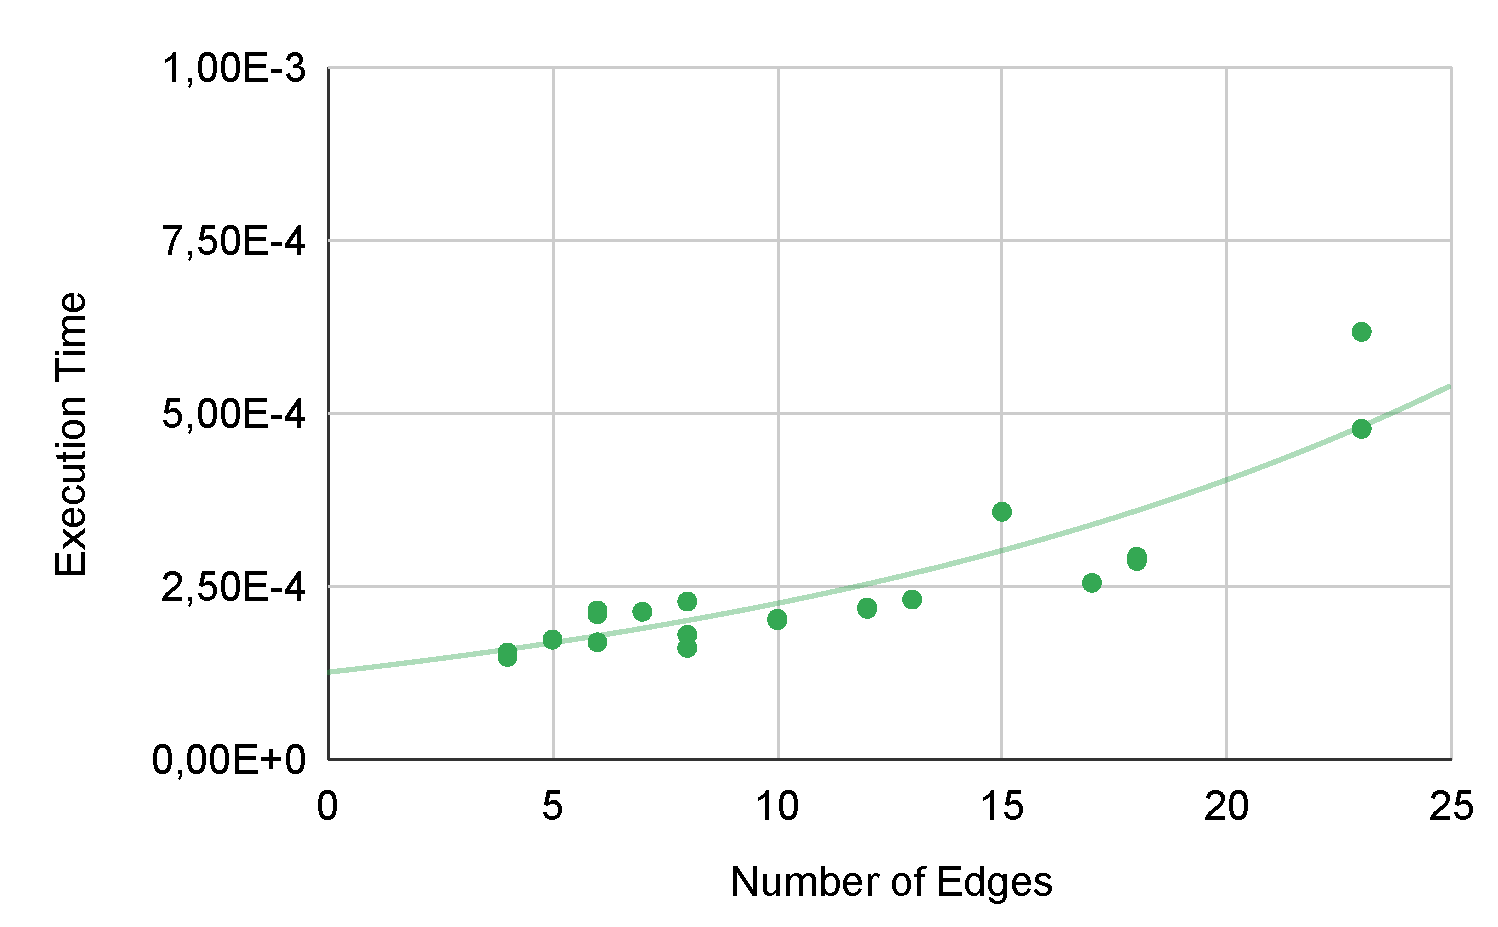
\includegraphics[width=0.9\linewidth]{figs/maxc-time.pdf}
    \caption{Correlation between number of edges and elapsed time for maximum connection greedy algorithm.}
    \label{fig:maxc-time}
\end{figure}

\newpage

\begin{figure}[!ht]
    \centering
    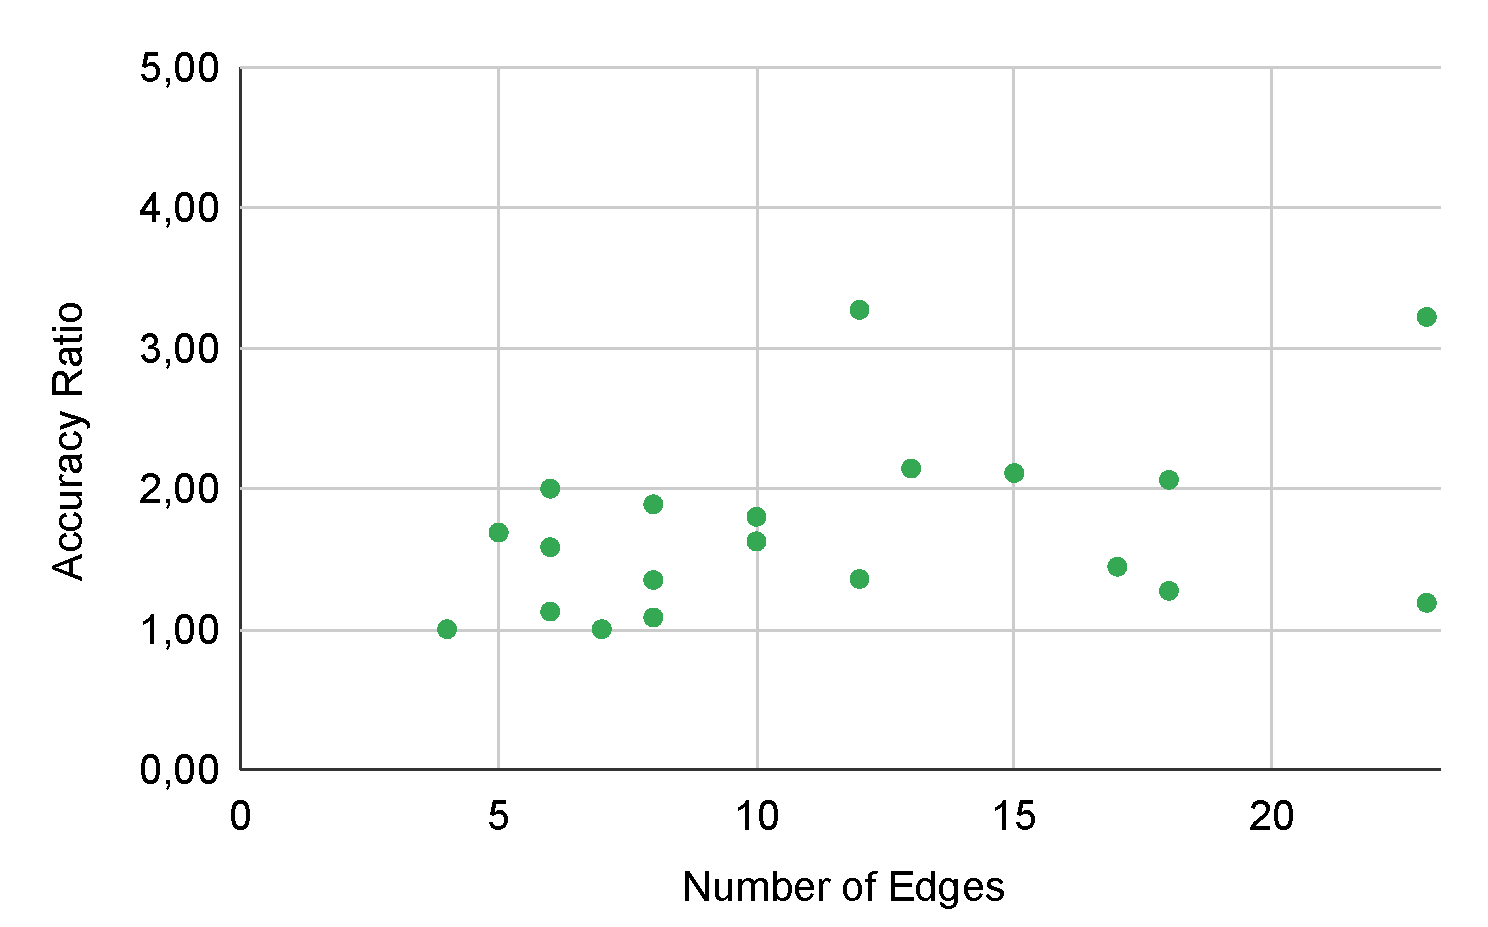
\includegraphics[width=0.9\linewidth]{figs/maxc-ratio.pdf}
    \caption{Correlation between number of edges and accuracy ratio for maximum connection greedy algorithm.}
    \label{fig:maxc-ratio}
\end{figure}

For the Chaurasia-Singh greedy heuristics, the results obtained are presented in \autoref{tab:chaurasia-table}, \autoref{fig:chaurasia-sol}, \autoref{fig:chaurasia-time}, and \autoref{fig:chaurasia-ratio}. 
The columns for \autoref{tab:chaurasia-table} are equal to the ones in \autoref{tab:minw-table}.
The data shows that the number of solutions tested grows with the number of edges, similar to the previous heuristics.
As with the previous algorithms, the correlation between the elapsed time and the number of edges presents a form of a $nlog_2(n)$ function, further verifying the hypothesis formed in \autoref{eq:greedy-big-o}.
The accuracy ratio for this algorithm is smaller then the two previous one.
This fact allows to affirm that this heuristics is more accurate than the preceding.

\newpage

\begin{table}[ht!]
\caption{Results from Chaurasia-Singh greedy algorithm}
\label{tab:chaurasia-table}
\resizebox{0.5\textwidth}{!}{%
\begin{tabular}{ccccccc}
\multirow{3}{*}{V} & \multirow{3}{*}{p} & \multirow{3}{*}{E} & \multirow{3}{*}{\begin{tabular}{c} Execution \\ Time (s) \end{tabular}} & \multirow{3}{*}{\begin{tabular}{c}\# of\\ Solutions\\Tested\end{tabular}} & \multirow{3}{*}{\begin{tabular}{c} Accuracy \\ Ratio \end{tabular}}\\ 
& & & & & & \\
& & & & & & \\
\hline
4 & 0.125 & 4 & 1,61E-04 & 1 & 1,80 \\
4 & 0.25 & 6 & 2,28E-04 & 2 & 1,00 \\
4 & 0.5 & 6 & 2,04E-04 & 2 & 1,00 \\
4 & 0.75 & 6 & 2,13E-04 & 2 & 1,00 \\
5 & 0.125 & 4 & 1,51E-04 & 1 & 1,00 \\
5 & 0.25 & 6 & 2,38E-04 & 2 & 1,00 \\
5 & 0.5 & 7 & 2,28E-04 & 2 & 1,00 \\
5 & 0.75 & 8 & 2,48E-04 & 2 & 1,00 \\
6 & 0.125 & 5 & 2,19E-04 & 2 & 1,50 \\
6 & 0.25 & 8 & 2,14E-04 & 3 & 1,61 \\
6 & 0.5 & 12 & 2,31E-04 & 3 & 1,00 \\
6 & 0.75 & 13 & 2,38E-04 & 3 & 1,00 \\
7 & 0.125 & 6 & 1,87E-04 & 3 & 1,00 \\
7 & 0.25 & 10 & 2,10E-04 & 3 & 1,60 \\
7 & 0.5 & 15 & 3,74E-04 & 3 & 1,56 \\
7 & 0.75 & 18 & 3,15E-04 & 3 & 1,27 \\
8 & 0.125 & 8 & 1,90E-04 & 3 & 1,00 \\
8 & 0.25 & 12 & 2,28E-04 & 3 & 1,00 \\
8 & 0.5 & 18 & 2,84E-04 & 3 & 1,31 \\
8 & 0.75 & 23 & 5,49E-04 & 4 & 1,75 \\
9 & 0.125 & 10 & 2,21E-04 & 3 & 2,13 \\
9 & 0.25 & 17 & 2,81E-04 & 3 & 2,56 \\
9 & 0.5 & 23 & 6,62E-04 & 3 & 4,44
\end{tabular}%
}
\end{table}

\begin{figure}[!ht]
    \centering
    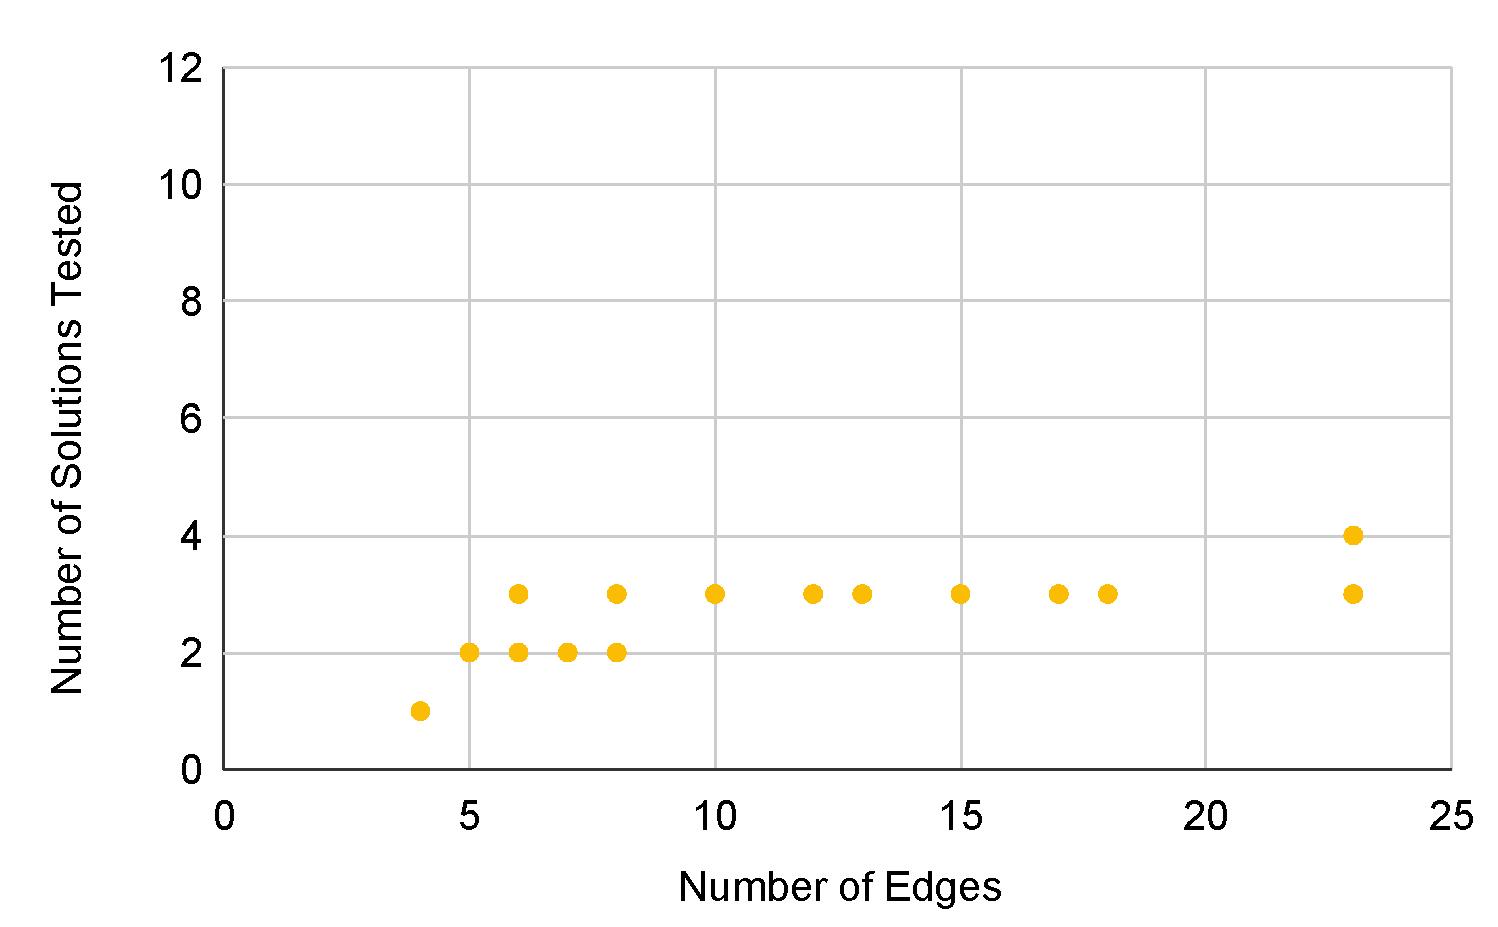
\includegraphics[width=0.9\linewidth]{figs/chaurasia-solutions.pdf}
    \caption{Correlation between number of edges and number of solutions tested for Chaurasia-Singh greedy algorithm.}
    \label{fig:chaurasia-sol}
\end{figure}


\begin{figure}[!ht]
    \centering
    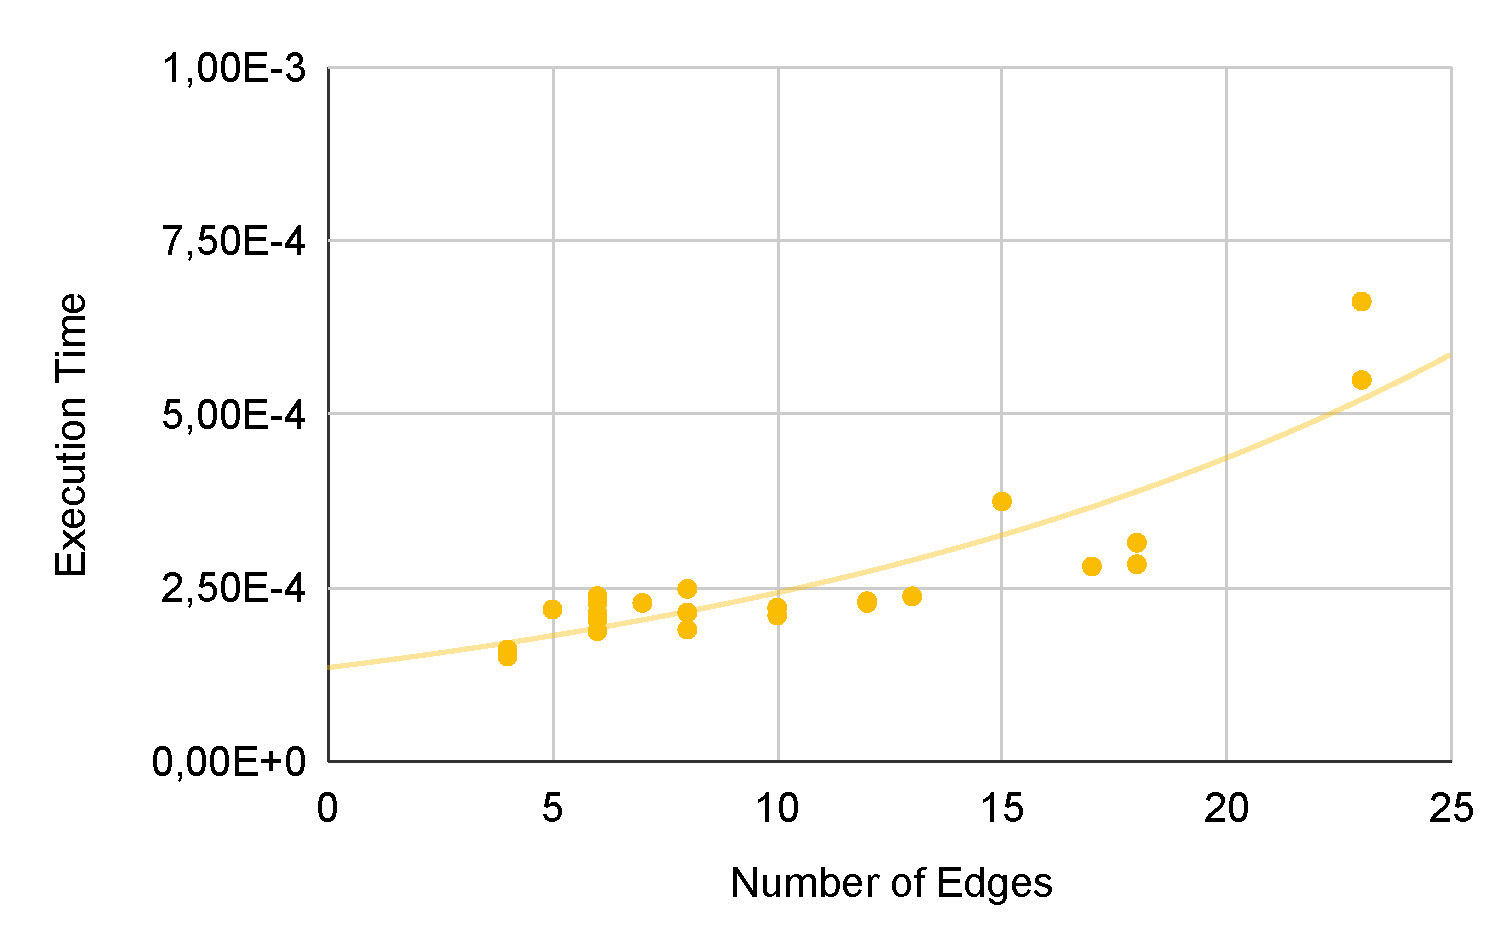
\includegraphics[width=0.9\linewidth]{figs/chaurasia-time.pdf}
    \caption{Correlation between number of edges and elapsed time for Chaurasia-Singh greedy algorithm.}
    \label{fig:chaurasia-time}
\end{figure}

\newpage

\begin{figure}[!ht]
    \centering
    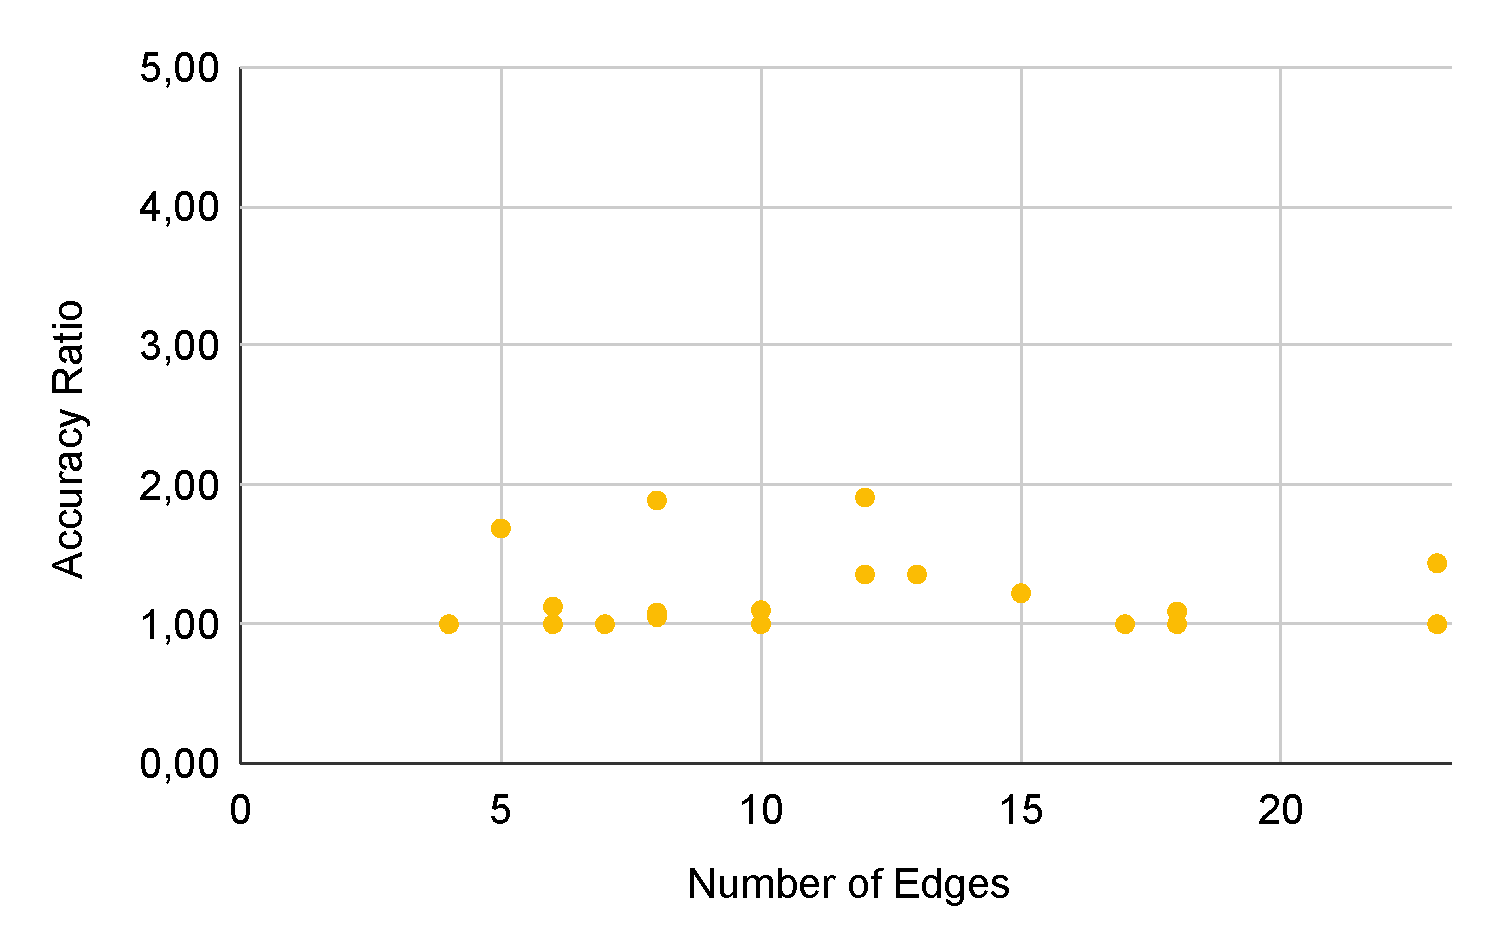
\includegraphics[width=0.9\linewidth]{figs/chaurasia-ratio.pdf}
    \caption{Correlation between number of edges and accuracy ratio for Chaurasia-Singh greedy algorithm.}
    \label{fig:chaurasia-ratio}
\end{figure}
\section{Conclusions}\label{section:conclusions}
In this report, four different algorithm to solve the minimum weight dominating set problem were proposed.
The first one is an exhaustive search algorithm, which based on its formal analysis it can be concluded that it is time-consuming but it guarantees an optimal solution.
The next three are greedy algorithms, which based on their formal analysis, they take less time than the exhaustive one, however, the solution is not guaranteed to be optimal.
The greedy algorithm are based on three different choices: choosing the edges with minimum weigh, choosing the edges with maximum number of connections, and choosing the edges with the largest ratio between the weight of adjacent edges and the weight of the edge itself.

Results prove that the exhaustive search and the greedy algorithms follow the behavior defined by their formal analysis.
It is also verified that the most accurate greedy algorithm is the one based on the work of Chaurasia and Singh.

Possible future work on this subject is the testing of exhaustive search in more complex graphs using better hardware, to further verify if it follows its formal analysis.
Another possible problem to tackle is the sorting in the greedy algorithms.
Currently, the sorting used was already created, giving the author no control over it, including not being able to verify how many basic operations it performed.
Still regarding the greedy algorithms, a n-log-n regression could be done on the data retrieved from these algorithms, to verify if it follows their formal analysis

\bibliography{references.bib}
% \bibliography{...} % use a field named url or \url{} for URLs
% Note: the \bibliographystyle is set automatically

\end{document}
